	\section{Factor graph}

	Un \textit{factor graph} è un grafo che rappresenta la fattorizzazione di una funzione, e si presta particolarmente per rappresentare i fattori di una distribuzione di probabilità. In un \textit{factor graph} un fattore che è $0$ oppure $1$ viene chiamato \textit{constraint}. 

	Gli elementi grafici che compaiono sono:
		\begin{itemize}
			\item un unico nodo quadrato per ogni fattore $f_k$
			\item un unico nodo rotondo per ogni variabile $x_i$
			\item un collegamento tra un nodo variabile $x_i$ e un nodo fattore $f_k$ qualora la variabile $x_i$ compaia nel fattore $f_k$ 
		\end{itemize}
		Data una funzione 
		\begin{equation*}
			f(u,x,y,z,w)=f_1(x,y) \times f_2(u,x,z) \times f_3(y,w)
		\end{equation*}
		il corrispondente factor graph può essere rappresentato come segue:
		\begin{equation*}
		\begin{tikzpicture}
			\SetUpEdge[lw = 0.2pt, color = gray]
			\begin{scope}
				\tikzset{VertexStyle/.append style={rectangle}}
				\Vertex[L=$f_1$,x=2,y=4]{f1}
				\Vertex[L=$f_2$,x=2,y=0]{f2}
				\Vertex[L=$f_3$,x=6,y=4]{f3}
			\end{scope}
				\Vertex[L=$u$,x=0,y=0]{u}
				\Vertex[L=$x$,x=2,y=2]{x}
				\Vertex[L=$y$,x=4,y=4]{y}
				\Vertex[L=$z$,x=4,y=0]{z}
				\Vertex[L=$w$,x=6,y=2]{w}
			\Edge(u)(f2)
			\Edge(x)(f1)\Edge(x)(f2)
			\Edge(y)(f1)\Edge(y)(f3)
			\Edge(z)(f2)
			\Edge(w)(f3)
		\end{tikzpicture}
	\end{equation*}
		Nel nostro caso tuttavia è più conveniente usare un grafo bipartito, con tutti i nodi variabile da una parte e tutti i nodi fattori dall'altra, come rappresentazione della funzione: $f: \textbf{Hx}=\textbf{z}$.
	
	\subsection{Esempio}
	
	Esempio di una matrice per un codice a blocchi generato casualmente con i seguenti paramentri:
	
	\begin{itemize}
		\item lunghezza blocchi $N = 16$
		\item peso colonne $J  = 3$
		\item peso righe $K = 4$
	\end {itemize}
	La matrice risultante è $H \in M_{12 \times 16}$ ad elementi in $\left\{0,1\right\}$
	
	\begin{equation} \label{matrix}
		\begin{smallmatrix}
			1& & & & & &1& &1&1& & & & & &  \\
			 &1& & & &1& &1& & &1& & & & &  \\
			1& & & & & & & &1&1& &1& & & &  \\
			 & & &1& &1& & & & & &1&1& & &  \\
			 &1& & &1& & & & & & &1&1& & &  \\
			 &1& & & & &1& & &1& & &1& & &  \\
			 & & &1& & & &1& & & & & &1& &1 \\
			 & & & &1& & & &1& &1& & &1& &  \\
			 & &1&1& & &1& & & & & & &1& &  \\
			1& & & &1& & & & & & & & & &1&1 \\
			 & &1& & &1& & & & & & & & &1&1 \\
			 & &1& & & & &1& & &1& & & &1& 
		\end{smallmatrix}
	\end{equation}
	
	Concettualmente ciascuno degli $n$ bit partecipa a $J = 3$ degli $m$ checks, mentre ciascuno degli $m$ checks effettua la somma di $K = 4$ bits collegati.
	Graficamente possiamo rappresentare la matrice di controllo come un grafo bipartito, da una parte tutti i bits e dall'altra tutti i checks. Per esempio il grafo associato alla matrice \ref{matrix} è il seguente:
	
	\begin{equation*}
		\begin{tikzpicture}[scale=0.77]
			\SetUpEdge[lw = 0.2pt, color = gray]
			\begin{scope}
				\tikzset{VertexStyle/.append style={rectangle}}
				\Vertex[L=\textbf{$c_1$},x=2,y=1]{c1}
				\Vertex[L=$c_2$,x=3.2,y=1]{c2}
				\Vertex[L=$c_3$,x=4.4,y=1]{c3}
				\Vertex[L=$c_4$,x=5.6,y=1]{c4}
				\Vertex[L=$c_5$,x=6.8,y=1]{c5}
				\Vertex[L=$c_6$,x=8,y=1]{c6}
				\Vertex[L=$c_7$,x=9.2,y=1]{c7}
				\Vertex[L=$c_8$,x=10.4,y=1]{c8}
				\Vertex[L=$c_9$,x=11.6,y=1]{c9}
				\Vertex[L=$c_{10}$,x=12.8,y=1]{c10}
				\Vertex[L=$c_{11}$,x=14,y=1]{c11}
				\Vertex[L=$c_{12}$,x=15.2,y=1]{c12}
			\end{scope}
				\Vertex[L=$x_1$,x=1,y=5]{x1}
				\Vertex[L=$x_2$,x=2,y=5]{x2}
				\Vertex[L=$x_3$,x=3,y=5]{x3}
				\Vertex[L=$x_4$,x=4,y=5]{x4}
				\Vertex[L=$x_5$,x=5,y=5]{x5}
				\Vertex[L=$x_6$,x=6,y=5]{x6}
				\Vertex[L=$x_7$,x=7,y=5]{x7}
				\Vertex[L=$x_8$,x=8,y=5]{x8}
				\Vertex[L=$x_9$,x=9,y=5]{x9}
				\Vertex[L=$x_{10}$,x=10,y=5]{x10}
				\Vertex[L=$x_{11}$,x=11,y=5]{x11}
				\Vertex[L=$x_{12}$,x=12,y=5]{x12}
				\Vertex[L=$x_{13}$,x=13,y=5]{x13}
				\Vertex[L=$x_{14}$,x=14,y=5]{x14}
				\Vertex[L=$x_{15}$,x=15,y=5]{x15}
				\Vertex[L=\textbf{$x_{16}$},x=16,y=5]{x16}
			\begin{scope}				
				\path[every node/.style={sloped,anchor=south,auto=false, color=blue}, every path/.style={line width=0.6pt}]
				 	(c1)  edge[color=blue] node[above] {$\textbf{H}_{1,1}=1$} (x1)
				 	(c1)  edge[color=blue] node[below] {$\textbf{H}_{1,10}=1$} (x10);
				\SetUpEdge[lw = 0.6pt, color = blue]
				\Edge(c1)(x7)
				\Edge(c1)(x9)
			\end{scope}
			\Edge(c2)(x2)\Edge(c2)(x6)\Edge(c2)(x8)\Edge(c2)(x11)
			\Edge(c3)(x1)\Edge(c3)(x9)\Edge(c3)(x10)\Edge(c3)(x12)
			\Edge(c4)(x4)\Edge(c4)(x6)\Edge(c4)(x12)\Edge(c4)(x13)
			\Edge(c5)(x2)\Edge(c5)(x5)\Edge(c5)(x12)\Edge(c5)(x13)
			\Edge(c6)(x2)\Edge(c6)(x7)\Edge(c6)(x10)\Edge(c6)(x13)
			\Edge(c7)(x4)\Edge(c7)(x8)\Edge(c7)(x14)
			\begin{scope}
				\SetUpEdge[lw = 0.6pt, color = red]
				\path[-, line width=0.6pt] (c7)  edge[color=red] node[sloped,anchor=south,auto=false, above] {$\textbf{H}_{7,16}=1$} (x16);
				\Edge(c10)(x16)
				\Edge(c11)(x16)
			\end{scope}
			\Edge(c8)(x5)\Edge(c8)(x9)\Edge(c8)(x11)\Edge(c8)(x14)
			\Edge(c9)(x3)\Edge(c9)(x4)\Edge(c9)(x7)\Edge(c9)(x14)
			\Edge(c10)(x1)\Edge(c10)(x5)\Edge(c10)(x15)
			\Edge(c11)(x3)\Edge(c11)(x6)\Edge(c11)(x15)\
			\Edge(c12)(x3)\Edge(c12)(x8)\Edge(c12)(x11)\Edge(c12)(x15)
		\end{tikzpicture}
	\end{equation*}
	
	Nel grafo viene evidenziato il fatto che un \textit{check} effettua la somma di quattro bits ($c_1$ con i collegamenti blu), e un singolo bit del blocco partecipa a tre \textit{checks} ($x_{16}$ con i collegamenti in rosso). Esiste un collegamento tra $c_m$ e $x_n$ quando $\textbf{H}_{mn}=1$.